\documentclass[a4paper]{article}
\usepackage{polski}
\usepackage[utf8]{inputenc}
\usepackage{secdot}
\sectiondot{subsection}
\usepackage{graphicx}
\usepackage{float}
\usepackage{listings}

\title{Komunikacja wieloprocesowa w języku Linda realizowana przy pomocy pamięci współdzielonej oraz semaforów}
\author{Michał Sypetkowski, Marcin Waszak, Łukasz Wlazły}
\date{}

\begin{document}
	\maketitle
	\newpage

	\section{Treść zadania}
	Komunikacja między-procesowa w Lindzie realizowana jest poprzez wspólną dla wszystkich procesów przestrzeń krotek.
    Krotki są arbitralnymi tablicami dowolnej długości składającymi się z elementów 2 typów podstawowych: \texttt{string}, \texttt{integer}.
    Przykłady krotek: \texttt{(1, "abc", "xyz")}, \texttt{(10, "abc")}.
    Funkcja \texttt{output} umieszcza krotkę w przestrzeni.
    Funkcja \texttt{input} pobiera i atomowo usuwa krotkę z przestrzeni przy czym wybór krotki następuje poprzez dopasowanie wzorca-krotki.
    Wzorzec jest krotką, w której dowolne składniki mogą być niewyspecyfikowane: "\texttt{*}" (podany jest tylko typ) lub zadane warunkiem logicznym. Przyjąć warunki: \texttt{==}, \texttt{<}, \texttt{<=}, \texttt{>}, \texttt{>=}. \\
    Przykład: \texttt{input(integer:1, string:*, string:"xy*")} - pobierze pierwszą krotkę z przykładu wyżej zaś: \texttt{input(integer:>2, string:"abc")} drugą.
    Operacja \texttt{read} działa tak samo jak \texttt{input}, lecz nie usuwa krotki z przestrzeni. Operacje \texttt{read} i \texttt{input} zawsze zwracają jedną krotkę.
    W przypadku, gdy wyspecyfikowana krotka nie istnieje, operacje \texttt{read} i \texttt{input} zawieszają się do czasu pojawienia się oczekiwanej danej.

	\section{Interpretacja treści zadania}
	\subsection{Interpretacja}
	\begin{enumerate}
		\item \texttt{ELEM\_SIZE}, \texttt{MAX\_TUPLES\_COUNT} - stałe edytowalne przed kompilacją, domyślnie 256 i 4096
		\item Krotki będą przechowywane w obszarze pamięci współdzielonej w postaci listy, do której dostęp będzie miał każdy proces korzystający z API dostępnego w tworzonej bibliotece.
		\item Pamięć współdzielona zawiera listę krotek.
		\item Każdy element listy ma wielkość \texttt{ELEM\_SIZE} bajtów.
		\item Każdy element listy zawiera: dane krotki, wskaźnik na następny element w liście oraz parę semaforów ("pisarz" oraz "czytelni") do synchronizacji.
		\item Wskaźnik na pierwszy element listy jest współdzielony i synchronizowany mechanizmem semaforów.
		\item Nowy element dodawany jest na koniec listy.
		\item Usuwanie elementu z listy wymaga 2 dostępów pisarza (dla 2 sąsiednich elementów - poprzednika i usuwanego).
		\item Odczytywanie polega na przeiterowanie się po liście aż odnajdzie się pasujący element (wymaga dostępów czytelnika dla obecnie czytanego elementu).
		\item Projekt zostanie wykonany w języku C++ (standard C++17).
		\item Pamięć współdzielona oraz semafory zostaną zrealizowane według standardu POSIX.
		\item Maksymalna liczba krotek jest stała - \texttt{MAX\_TUPLES\_COUNT}.
		\item Obszar pamięci na krotki będzie zawierał nagłówek określający ilość elementów krotki i typy jej elementów, a także wartości przesunięć względem początkowego adresu krotki. Wartości elementów będą stanowiły resztę obszaru.
	\end{enumerate}
	
	\subsection{Struktura danych w pamięci współdzielonej}
	\begin{figure}[H]
	\centering
	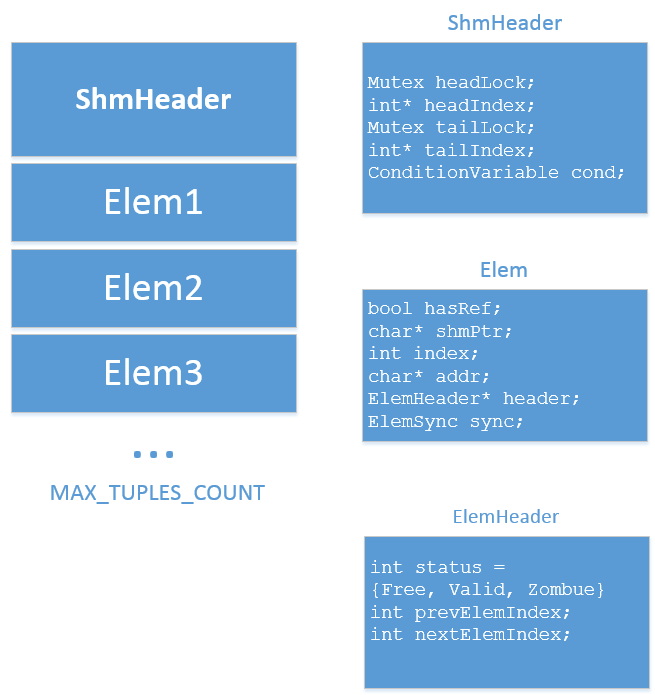
\includegraphics[width=130mm]{images/struct.png}
	\caption{Struktura danych znajdująca się w pamięci współdzielonej}
	\end{figure}


	\subsection{API}
	Użytkownik biblioteki ma do dyspozycji dwie główne klasy: \texttt{Tuple} oraz \texttt{Buffer}. Pozwalają one na wygodną implementację funkcjonalności oferowanej przez języka Linda. Ponadto udostępniono kilka klas pomocniczych: \texttt{QueryLexer}, \texttt{QueryParser}, \texttt{TupleParser}, \texttt{StringOrNumber}
	\subsubsection{Tuple}
	Uniwersalna abstrakcja dla krotek używanych wewnątrz Lindy. Klasa udostępnia trzy konstruktory: \\
	\begin{enumerate}
		\item \texttt{Tuple() = default}
		\item \texttt{Tuple(std::vector<StringOrNumber> values)} - ta wersja w szczególności pozwala na stworzenie poprawnej krotki przy użyciu następującej konstrukcji: \texttt{auto tuple = Tuple\{\{1, "two", 3, "four"\}\};}
		\item \texttt{Tuple(unsigned char* addr)} - dzięki tej konstrukcji biblioteka potrafi odczytać krotkę zapisaną w obszarze pamięci współdzielonej w surowej formie (jako ciąg bajtów)
	\end{enumerate}
	Każda istniejąca krotka może zostać rozszerzona dzięki metodzie \\ \texttt{void append(StringOrNumber value)}. \\
	Ponadto obiekt tej klasy potrafi zapisać krotkę, którą reprezentuje, bezpośrednio pod wskazany adres pamięci. Realizuje to funkcja \texttt{void write(unsigned char* addr) const}. \\
	Klasy \texttt{QueryLexer} oraz \texttt{QueryParser} pozwalają na analizę wzorca zadanego do metod i przetworzenie go do postaci par: typ - funkcja lambda, przy czym \texttt{QueryLexer} analizuje wzorzec jako ciąg znaków, natomiast \texttt{QueryParser} bazuje na tokenach zwróconych przez pierwszą z wymienionych klas. Zapis wzorców w formie par sprawia, że za pomocą metody \texttt{bool match(const QueryVec \&pattern)} krotka potrafi sprawdzić, czy jej zawartość odpowiada zadanemu wzorcowi.
	
	\subsubsection{Buffer}
	Abstrakcja dla obszaru pamięci, w którym zapisywane są krotki. Jedyny konstruktor \texttt{Buffer(const std::string \&shmName, bool initialized=true)} przyjmuje jako argument nazwę podaną przez użytkownika, która pozwala na jednoznaczną identyfikację obszaru pamięci w systemie. Dzięki temu w systemie może istnieć niezależnie wiele działających instancji do komunikacji w Lindzie. \\
	Umieszczono tu także metody \texttt{output}, \texttt{input} oraz \texttt{read}, które realizują funkcjonalność określoną w treści zadania. \\
	Obiekt klasy \texttt{Buffer} w czasie swojego życia może być wielokrotnie inicjalizowany i zamykany.
	
	\subsection{Interfejs użytkownika}
	Projekt, oprócz biblioteki realizującej funkcjonalność Lindy, zawiera kod wykorzystujący tę bibliotekę. W zbudowanym projekcie dostępny jest plik binarny \texttt{linda-communication}, który realizuje funkcje serwera i klienta (w zależności od wybranych parametrów).
	\\
	Pełny opis dostępny przy użyciu flagi "--help". Wszystkie operacje muszą mieć podany identyfikator pamięci - podawany przez parametr "--name". \\
	
	Jako pierwszy musi zostać uruchomiony serwer, ten tryb zapewnia opcja "--server". Uruchomienie serwera z dozwoloną nazwą utworzy obszar, do krótego będą mogli łączyć się klienci. Zamknięcie serwera spowoduje usunięcie obszaru, który utworzył. \\
	
	Klient ma do dyspozycji cztery polecenia: "--output", "--input", "--read" oraz "--timeout". Ostatnie polecenie pozwala na realizację czytania/wyjmowania krotki z ograniczeniem czasowym. Ponieważ wymagane jest, aby ciągi znakowe podawać w cudzysłowiu, argumenty, będące krotkami lub wzorcami, najlepiej podawać w apostrofach, np:\\ \texttt{./linda-communication -n "space" -o '(1, "ala ma kota", 3)'}.
	
	\subsection{Wykorzystane technologie}
	\begin{enumerate}
		\item Zgodnie z wymaganiami odnośnie do projektu, komunikacja oraz synchronizacja międzyprocesowa została zrealizowana przy pomocy pamięci współdzielonej oraz semaforów zgodnych ze standardem POSIX. Wybrano ten standard ze względu na dobrą dokumentację oraz intuicyjne API.
		\item Głównym językiem projektu jest C++ w wersji 17. Jest to najnowsza (oficjalnie wydana) wersja tego języka, oferująca wiele ciekawych rozwiązań, jak np. std::optional.
		\item Budowanie projektu wspiera narzędzie cmake.
		\item Analiza argumentów wywołania w aplikacji testowej oraz testy biblioteki zostały zaimplementowane z użyciem biblioteki boost. 
	\end{enumerate}
	

	\subsection{Obsługa błędów}
	Wszystkie sytuacje błędne będą sygnalizowane poprzez wartości zwracane z funkcji.
	Metoda \texttt{output} może zakończyć się na dwa sposoby: sukcesem lub porażką z powodu braku pamięci na nową krótkę. Sytuacje te zostaną zmapowane na wartości liczbowe i zwrócone do użytkownika.
	Metody \texttt{input} oraz \texttt{read} zwrócą krotkę, jeśli istnieje lub nic jeśli krotka pasująca do wyrażenia nie znajdzie się w buforze przez upłynięciem podanego czasu. Klasa \texttt{std::optional} z biblioteki standardowej pozwoli na bezpieczne obsłużenie obu sytuacji.



\end{document}
